\section{Auswertung}
\label{sec:Auswertung}
Für die Auswertung des vorliegenden Versuchs wurden experimentell, die in \autoref{fig:daten} aufgeführten, Messdaten ermittelt.

\begin{figure}
  \centering
  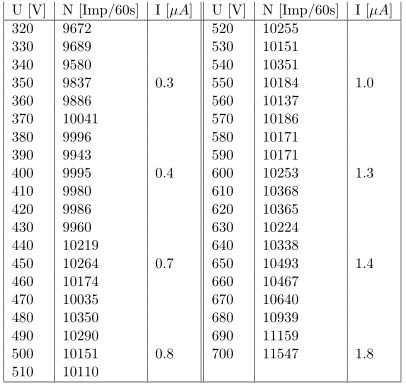
\includegraphics{content/daten.JPG}
  \caption{Messwerte \cite{sample}}
  \label{fig:daten}
\end{figure}

\subsection{Zählrohr-Charakteristik}
In \autoref{fig:plot} wurden die Messwerte mit Fehlerbalken (Messunsicherheiten $\Delta N = \sqrt{N}$) und die Plateau-Gerade graphisch dargestellt. Als Spannungsbereich für das Plateau wurde dabei $U=370V$ bis $U=570V$ gewählt. In diesem Bereich wurden die Messwerte an eine Gerade angepasst. Die Steigung der Ausgleichsgeraden ergibt sich zu $a=(1.084 \pm 0.320) Imp/(V*60s)$ und der y-Achsenabschnitt zu $b=(9614.609 \pm 155.153) Imp/60s$. Als Steigung für die Plateau-Gerade ergibt sich $(1,08 \pm 0.32) \%/100V$
\begin{figure}
  \centering
  \includegraphics{build/plot1.pdf}
  \caption{Messwerte zur Zählrohr-Charakteristik und Plateau-Gerade}
  \label{fig:plot}
\end{figure}

\newpage
\subsection{Abstand zwischen Primär- und Nachentladungsimpulsen}
Im Versuch wurde das in \autoref{fig:plot1} zu sehende Oszilloskopbild aufgenommen. Als Abstand zwischen Primär- und Nachentladungsimpulsen wurde hier $450 \mu s$ abgelesen.
\begin{figure}
  \centering
  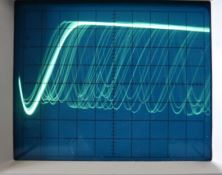
\includegraphics{content/oszill.JPG}
  \caption{Oszilloskopsaufnahme im Maßstab $100\mu s/DIV$ \cite{sample}}
  \label{fig:plot1}
\end{figure}

\subsection{Bestimmung der Totzeit}
Oszilloskop-Methode:
Mit der Oszilloskop-Methode wurde die Totzeit anhand von \autoref{fig:plot1} zu $T=90 \mu s$ abgelesen.
\newline
\newline
2-Quellen Methode:
Für die Bestimmung der Totzeit mit der 2-Quellen-Methode wurden die in \autoref{tab:mess2} aufgeführten Messwerte ermittelt. Die Totzeit kann dann wie im Theorieteil beschrieben nach \autoref{eqn:totzeit-naeherung} berechnet werden. Mit den Messunsicherheiten $\Delta N = \sqrt{N}$ und der Gaußschen Fehlerfortpflanzung ergibt sich dann für die Totzeit $T=115 \pm 47 \mu s$.
\begin{table}
  \centering
  \caption{Zählraten zur 2-Quellen-Methode}
\label{tab:mess2}
  \sisetup{table-format=2.1}
  \begin{tabular}{c c c c}
  \toprule
  Quelle & $N [\frac{Imp}{120s}]$ \\
  \midrule
  1     & 96041  \\
  2     & 76518 \\
  1 + 2 & 158479 \\
  \bottomrule
  \end{tabular}
  \end{table}
  \newpage
  \subsection{Pro Teilchen vom Zählrohr freigesetzte Ladungsmenge}
  Die pro einfallendem Teilchen im Zählrohr freigesetzte Ladung kann mit $Z=\frac{I}{\epsilon_0 N}$ berechnet werden. Mit den ermittelten Messwerten können so also Wertepaare für $Z$ zu verschiedenen Zählrohrspannungen $U$ ermittelt werden. Die Ablesegenauigkeit des Amperemeters beträgt $\Delta I= 0.05 \mu A$. Die so ermittelten Werte für Z sind in \autoref{fig:plotd} in Einheiten der Elementarladung abhängig von der Zählrohrspannung U dargestellt.
  \begin{figure}
    \centering
    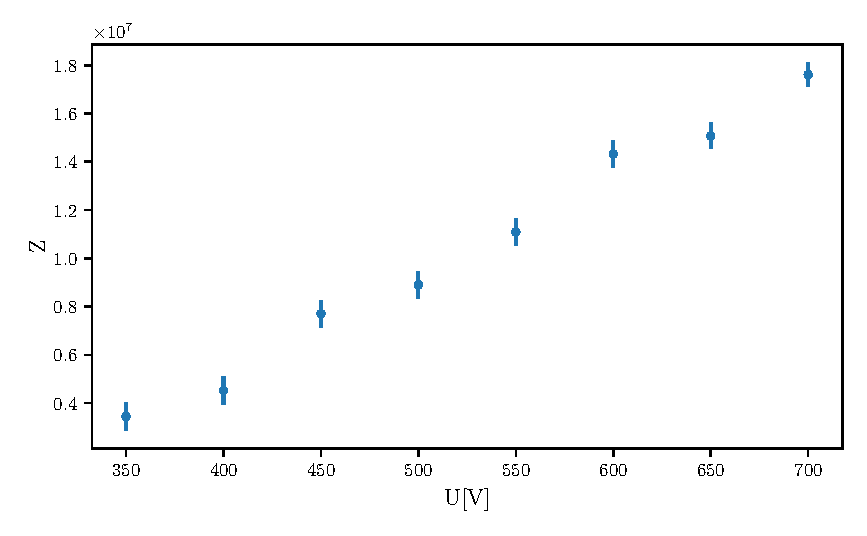
\includegraphics{build/plotd.pdf}
    \caption{Pro einfallendem Teilchen im Zählrohr freigesetzte Ladung in Abhängigkeit von der Zählrohrspannung}
    \label{fig:plotd}
  \end{figure}